\chapter{Proposed System} \label{chap:proposed_sys}

This chapter is dedicated to the presentation and overall explanation of the developed system, highlighting its capabilities, the used methodologies and overall design strategies. 
The system will be presented in two distinct sections. The first component is the HDL module, which falls into the spectrum of hardware design and requires insight on hardware development and good practices. The second section relies on software development to complement the functionality of the mentioned module, so that is possible to deliver the desired result.

\section{HDL Module Architecture} \label{subsec:HDL module}

The system which is proposed to be implemented in this research work has as input 4 signals which are received by each hydrophone of the array, and outputs an average phase difference between all combinations of pairs of hydrophones. 

- ver regras basicas de hardware development
- sustema sincrono, available clock cycles globais
- hardware limitations
- tamanho das entradas


\begin{enumerate}
	\item Hilbert Filter
	\item Cordic
	\item phasediff
	\item phasemean
\end{enumerate}

\subsection{Hilbert Filter}


\begin{eqnarray}
H(f)(t) = \frac{1}{\pi}\int_{-\infty}^{\infty}\frac{f(\tau)}{t-\tau}d\tau
\label{eq:hilbert_integral}
\end{eqnarray}

\begin{eqnarray}
&Imag_0 = x_{-1}*c_1 + x_{-3}*c_3 + x_{-5}*c_5 + x_{-7}*c_7
\label{eq:hilbert_imeq}
\end{eqnarray}

\begin{eqnarray}
&Real_0 = x_{-4} 
\label{eq:hilbert_reeq}
\end{eqnarray}

- matematica brevemente, equação base, resposta impulsional, ganho, coeficientes e ordem usada
\\
- schematics 
\\
- explicar design decisions
\\
- descrever brevemente flow do sinal no hardware

\subsection{Cordic}
- descriçao do que faz, matematica (?)
\\
- entradas e saídas, clocks, ROM

\subsection{phasediff}
-pequeno esquema 
\\
- 1 sub

\subsection{phasemean}
- pequeno esquema
\\
- N accumulated
\\
---------
\\
apresentar esquema global menos pormenorizado


\subsection{Phase Ambiguity}

When the information about the time of flight of a signal is available, it is relatively easy to estimate the range of the communication since there can be a direct conversion between them. However, when dealing with phase differences, there is no exact time notion, so it is necessary to start by defining a reference point. 

Considering sinusoidal signals, when we have an array with four hydrophones spatially placed to form a 3D layout, the signal that is arriving to each  hydrophone in different times consequently have different phases. However, since sinusoidal signals are periodic, this means that for different signal periods the same phase value is observed, i.e. the phase is ambiguous. It is possible to observe this phenomenon in figure \ref{fig:phasediff}. In this illustration, $\alpha$ represents the observable phase difference of hydrophone $H_4$ to the reference point $H_1$. However, the actual phase difference which is intended to obtain, $\Delta p_4$, is one period of the signal, $\lambda$, added to the observable phase $\alpha$.

\begin{figure}[!htbp]
	\centering
	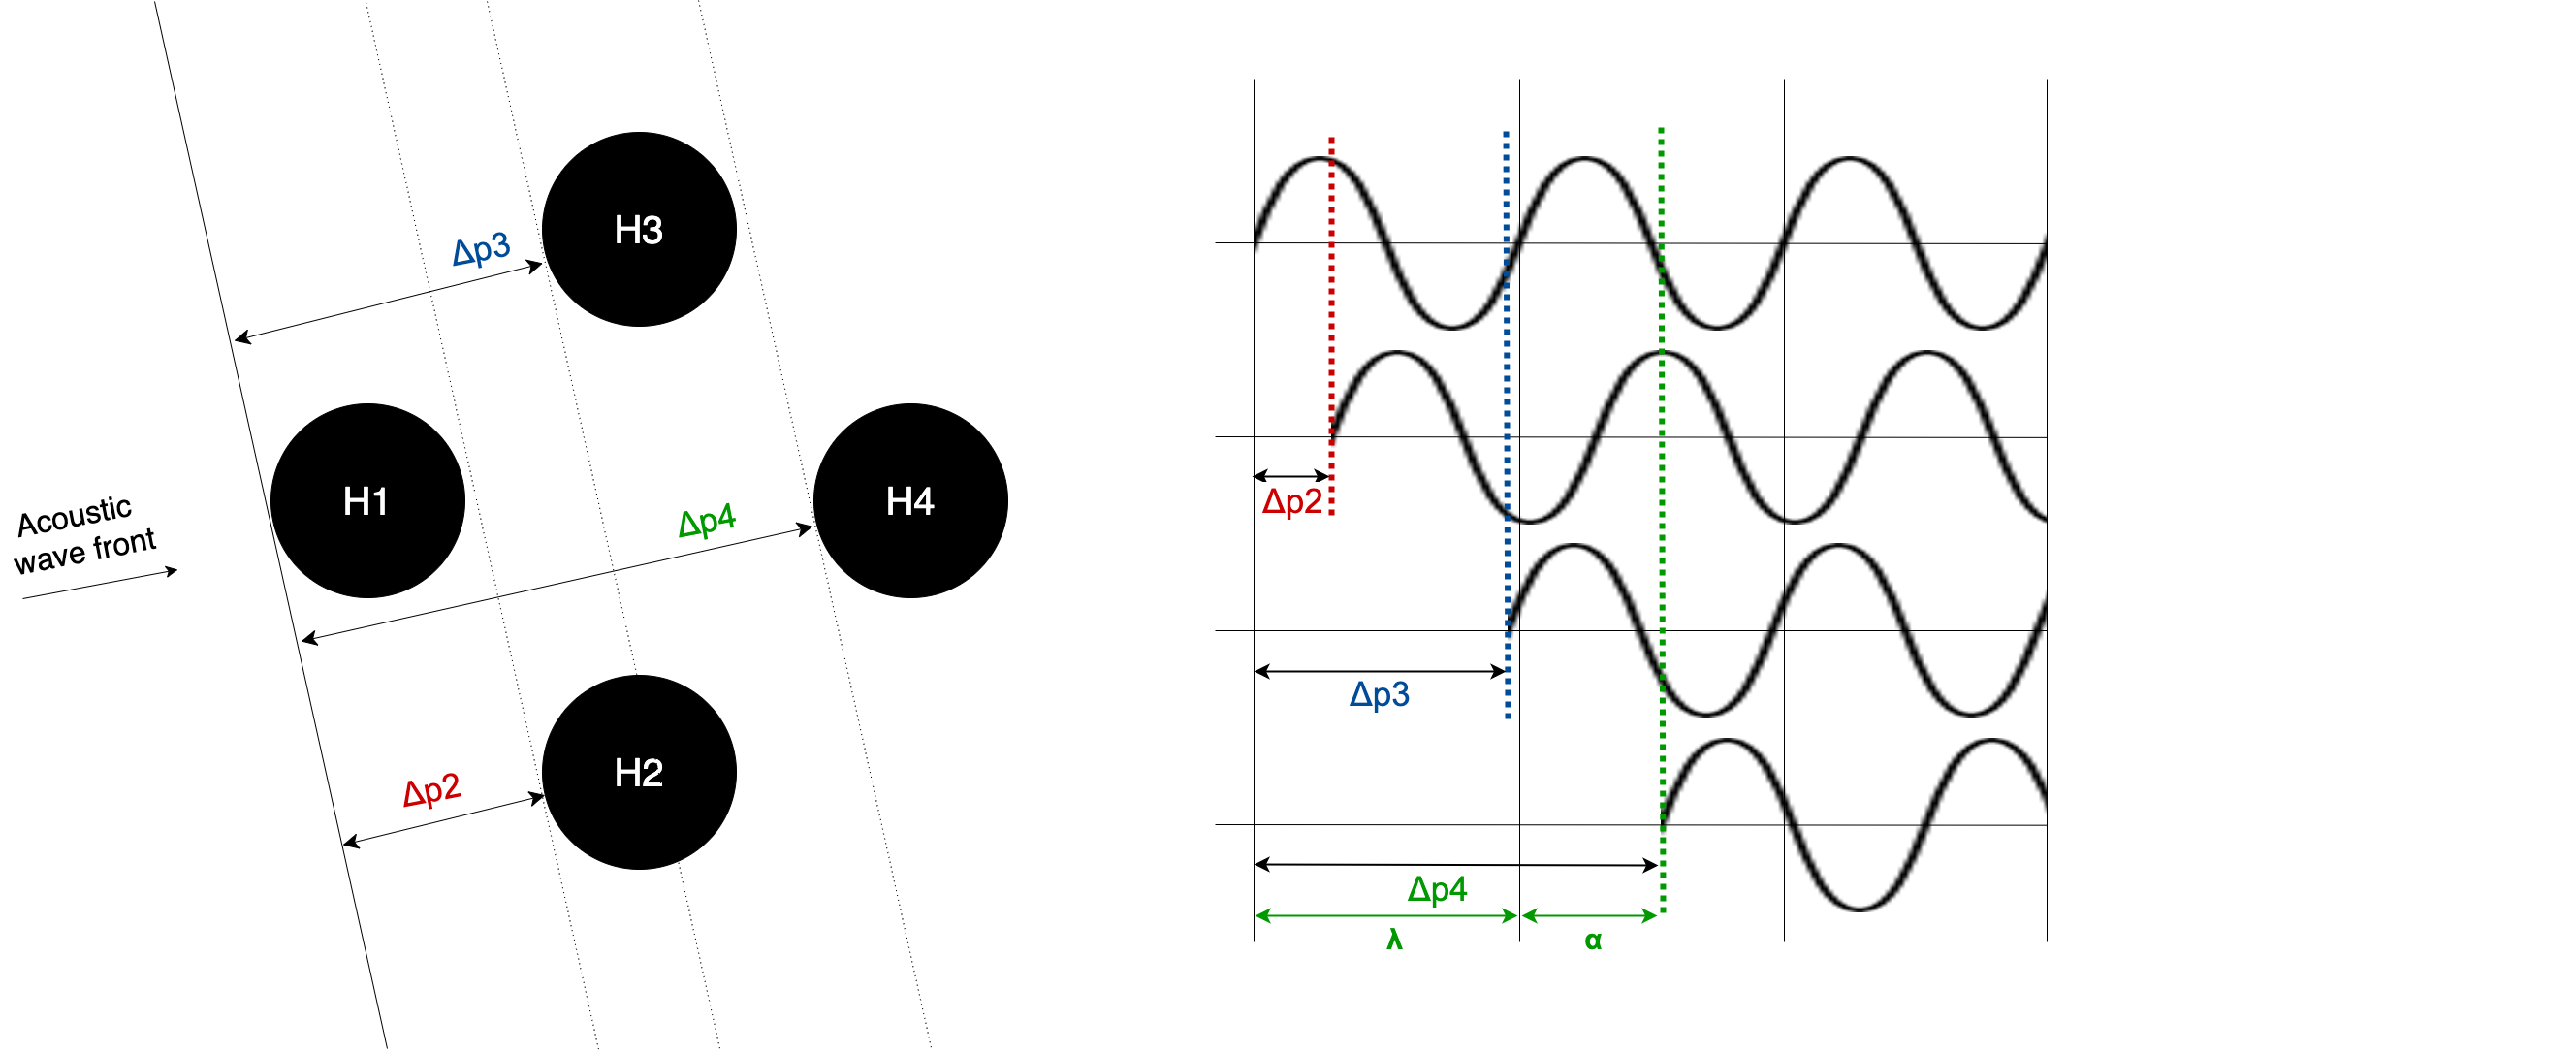
\includegraphics[width=1.2\textwidth]{figures/phase-diff}
	\caption{Phase difference to reference point and phase ambiguity}
	\label{fig:phasediff}
\end{figure}

For this reason, it is crucial to consider that the phase difference is given by the obtained phase value added by the number of periods ahead from the considered reference period.

In the system under study, the sent signals work with a operation frequency of 24.4 $kHz$. The corresponding signal period is $T = \frac{1}{24400} $ seconds which, considering the underwater acoustic speed \textit{c} equal to a standard 1500 $m/s$, the wavelength is approximately equal to $\lambda = \frac{T}{c} = 6.1 cm$. Having this into consideration, after obtaining the time of arrival to each hydrophone given by the cross correlation instances, besides the reference one, it is possible to conclude if the phase shift is superior to one period by analyzing if the time difference is greater than the duration of one period \textit{T}. In figure \ref{fig:phasediff}, each mentioned time difference between $H_1$ and $H_2$, $H_3$ and $H_4$ is converted to the corresponding phase differences $\Delta p_2$, $\Delta p_3$ and $\Delta p_4$.

%From this phase differences, it is possible to estimate the angle of arrival from which the acoustic wave is coming from by comparing all pairs of hydrophones: H1-H2, H1-H3, H1-H4, H2-H3, H2-H4, H3-H4. 

One possibility to solve phase ambiguity in this system would be to place the four hydrophones with a baseline spacing inferior to $\frac{1}{2}$ of a wavelength, since the maximum reached by phase difference is 180 degrees. This way it would be possible to immediately deduce the phase difference since it would always be contained in one period. However, positioning the hydrophones closer together leads to smaller TDoA values,causing a consequent increase on the estimation error due to varying environment conditions (briefly enumerated in \ref{subsec: acoustic-channel}). Additionally, since the hydrophones to be used in this system have a corresponding diameter of roughly half of a wavelength, they would not allow to execute the mentioned configuration and so this possibility will not be contemplated.

In order to compensate this phase ambiguity, a simple relationship was developed which allows to calculate the absolute time difference between when a signal is received by hydrophone A and the moment the same signal is received by a further hydrophone B. This uses the time stamps obtained by the correlation peaks and the additional phase difference, that is determined in parallel, so that the measurement is more accurate. Equation \ref{eq:phase-amb} translates this relation, where $T_A$ and $T_B$ are the moments a signal is perceived by hydrophones A and B respectively, $t_1$ and $t_2$ are the moments corresponding to the correlation peaks of the signal in hydrophone A and B respectively, $T$ is one period of the signal, $\theta_A$ and $\theta_B$ are the phases in 

\begin{eqnarray}
& T_B - T_A = round(\frac{t_2-t_1}{T}) - (\theta_B - \theta_A)
\label{eq:phase-amb}
\end{eqnarray}


\section{Angle of Arrival Estimation} \label{subsec:AoA}

In order to estimate the position of an acoustic source, it is used the phase differences obtained from the system explained in the previous section and additional mechanisms that will be better explained in the present section.

For the estimation of the position in 3D space , a multilateration approach was used. As explained in \ref{subsec:multilateration}, the concept of multilateration implies that relative distances between a target and multiple sensors are combined in order to locate the target. In the present case, four sensors are used in a defined configuration in three dimensional space. By using two sensors, the location solutions are contained in a sphere of possibilities. 

\subsection{Theoretical considerations}
%---Hyperbole------------------------------
In order to estimate the location of an acoustic source we take into account the phase differences between each pair of hydrophones, carefully explained in  section \ref{subsec:HDL module}. These phase differences combined with the ToF obtained from arriving acoustic signals can be translated into periods of the signal and thus into relative distances. To better understand the location estimation of the acoustic source we can initially adopt the two dimensional scenario of figure \ref{fig:hyper}. 

Considering two hydrophones at known relative positions $(-f,0)$ and $(f,0)$, we can model all possible acoustic source locations for a specific time of arrival difference through hyperbolas. This is due to the fact that, by definition, the sum of the distances from the focus of each hyperbole, where each hydrophone is placed, to any point of the hyperbolic geometry corresponds to a constant value. 
This means that, in figure \ref{fig:hyper}, any point $(x,y)$ that is contained in the hyperbole corresponds to a constant $|d_2-d_1|$ value which, after some formulation, is in fact equal to $2*v$ or the distance between the vertexes of each hydrophone's hyperbola. Therefore, it is possible to trace a hyperbole that represents the positions of the target in space both based on their distance and the signal's ToA. In the exceptional case where $d_3=d_4$, we can observe that the possible positions are represented by an equidistant straight line to each hydrophone, such as the y axis.

\begin{figure}[!htbp]
	\centering
	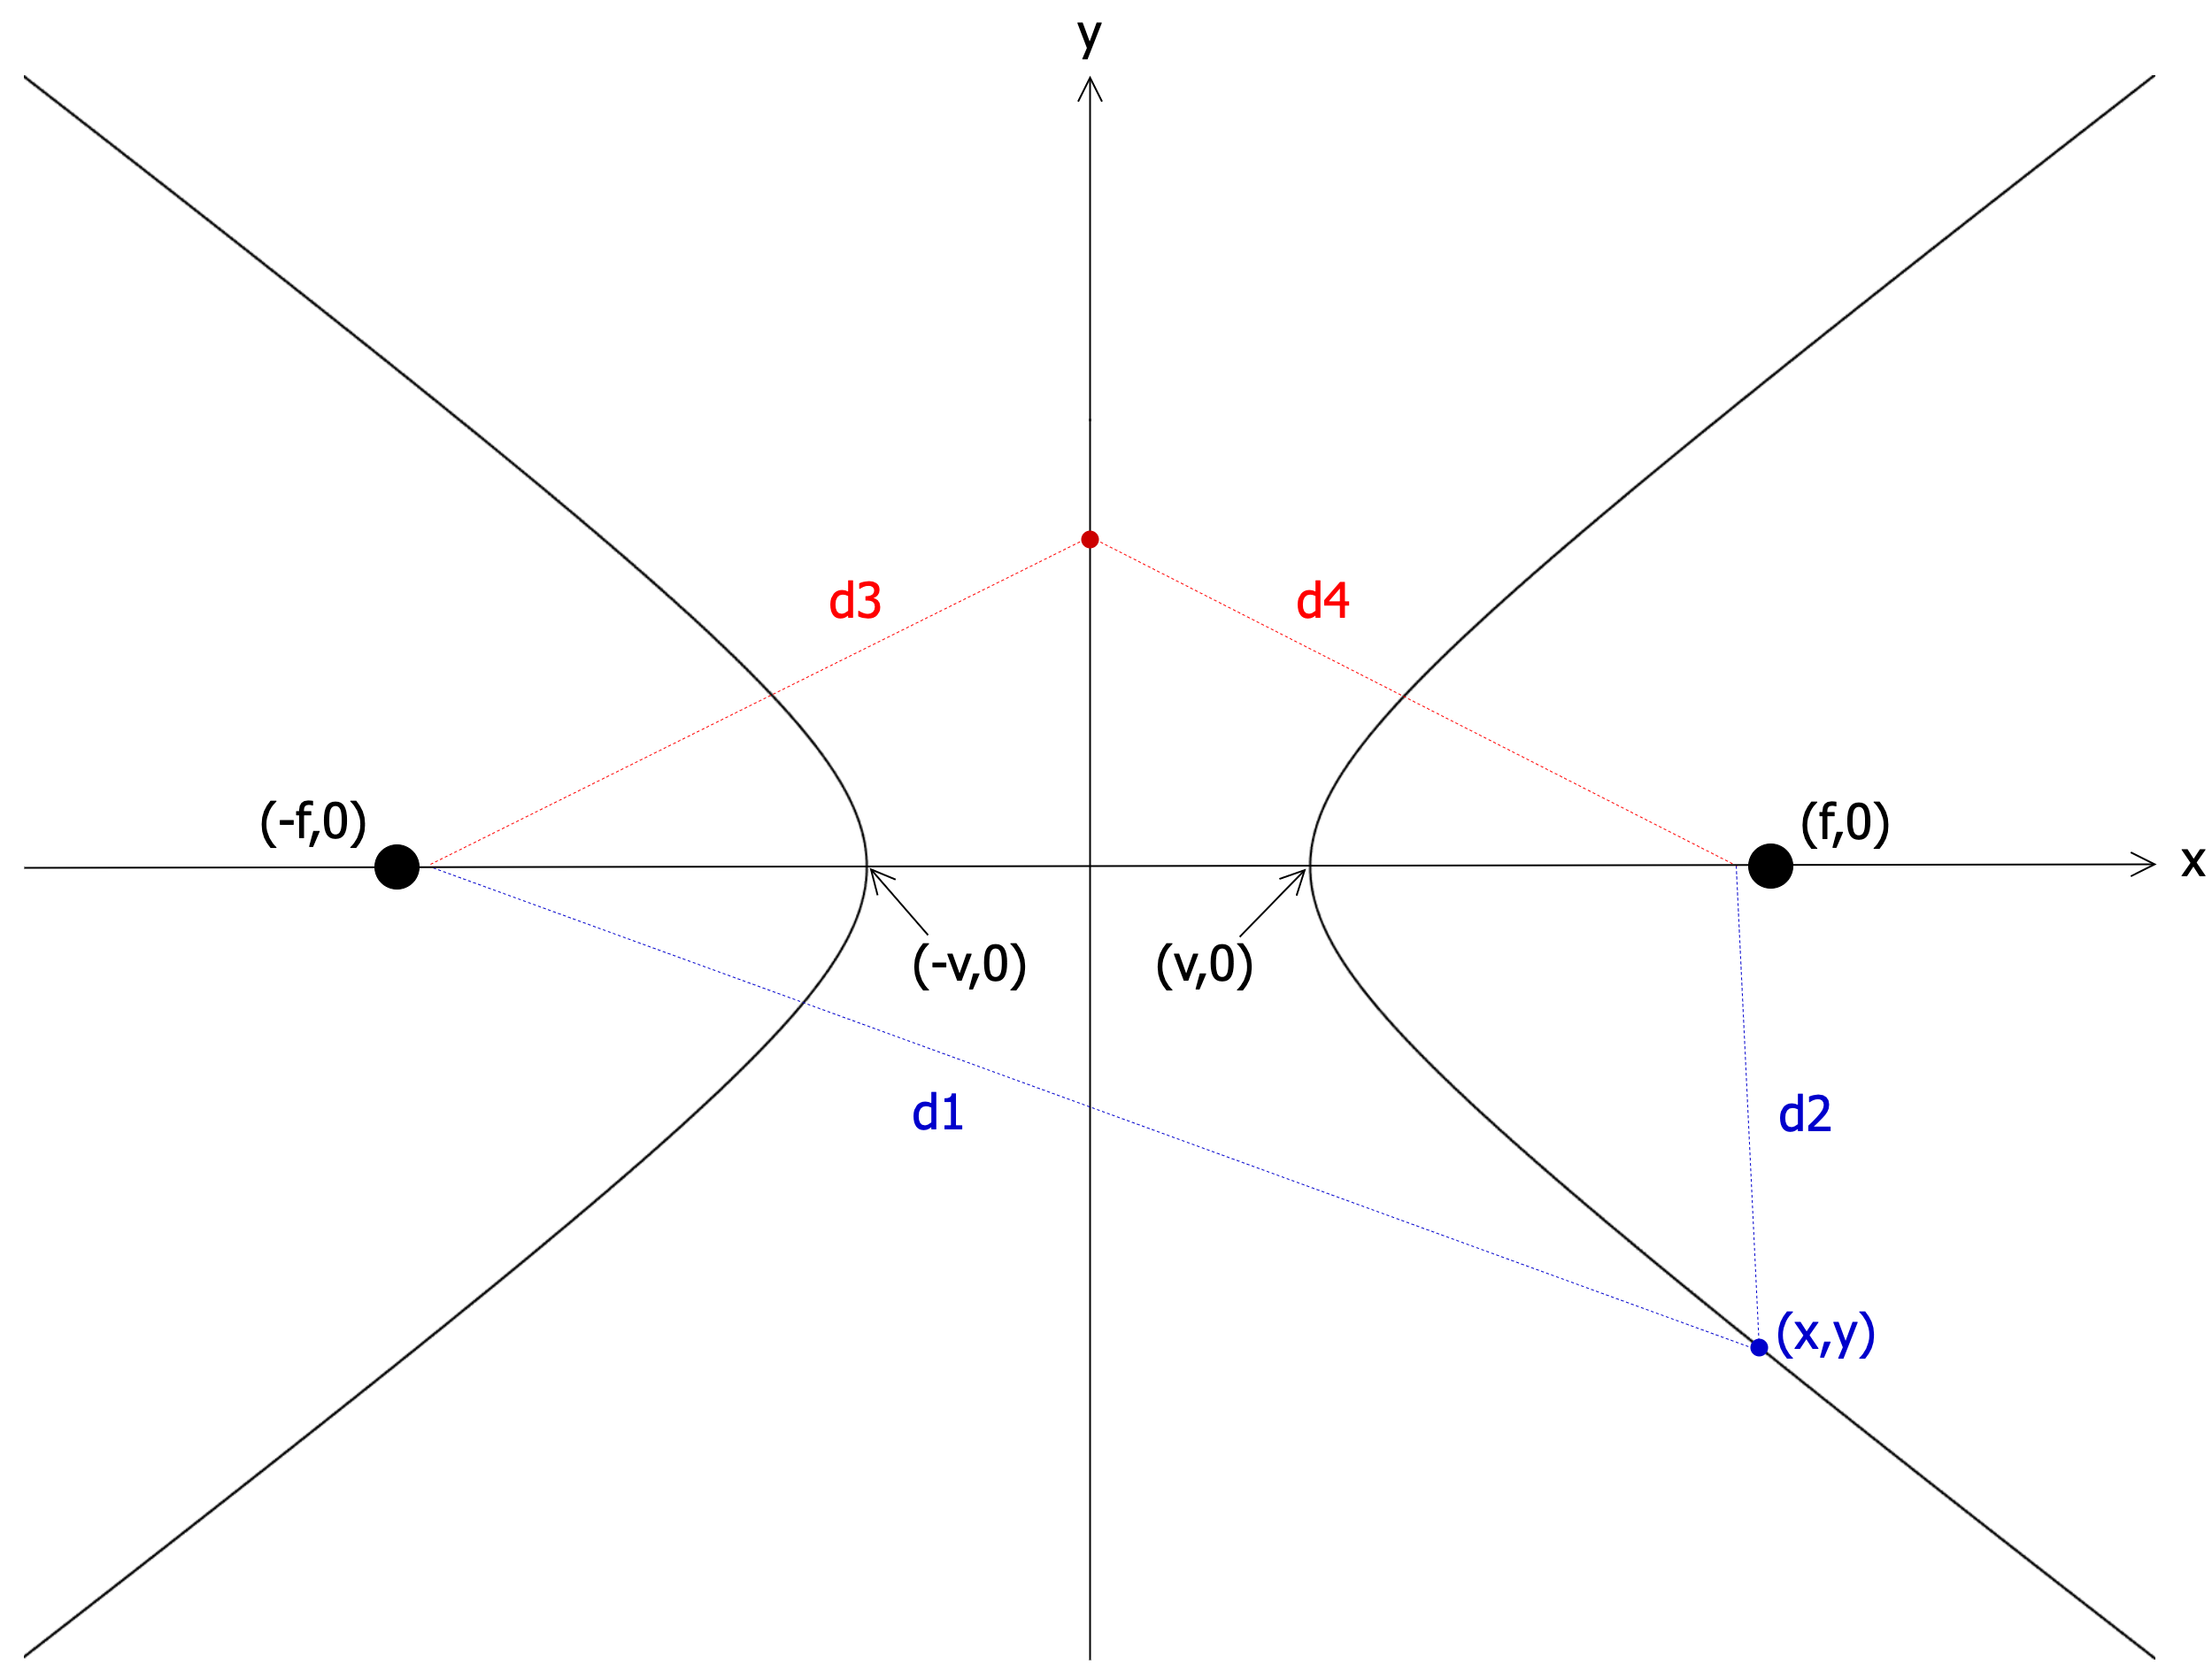
\includegraphics[width=0.8\textwidth]{figures/hyperbole-dist}
	\captionsetup{justification=centering,margin=2cm}
	\caption{Hyperbolic representation of acoustic source position possibilities in relation to ToA to two hydrophones}
	\label{fig:hyper}
\end{figure}

Following this idea, it is possible to model the distance of one sensor to the target based on the known distance of a second sensor to the same target. This is to say that for two sensors with a known relative position where hydrophone 1 is the closer to the target, the distance from hydrophone i to the target, $D_i$, is given by the distance of hydrophone j to the target, $K_{D_j}$, added by the time difference of arrival, $\Delta t_{ij}$, multiplied by the propagation velocity, $v_p$. Overall, this relationship can be translated by equation \ref{eq:dist_to_target}.

\begin{eqnarray}
& D_i = K_{D_j} + \Delta t_{ij} * v_p
\label{eq:dist_to_target}
\end{eqnarray}

Therefore, the same logic can be applied for multiple hydrophones. In the present work, in which it is consider a system with four hydrophones, a synchronization mechanism allows to determine the ToF of signals between the transceiver and the hydrophones. However, in order to simplify the synchronicity and decrease error that arise from it, the module that precisely computes the phase differences of the received signal in the hydrophones is used so that is possible to apply the relationship in \ref{eq:dist_to_target}. Consequently, a better angle of arrival estimation can be achieved when using this approximation than if all four times of flight are used for the same purpose. 


- explicar calculos de angulo de chegada (scipt + matematica) com base nas posições dos hydrophones e do angulo de chegada

- por simulação, conclui que para distancias muito longe (quantizar) não faz diferença ter o TOA e basta os TD OA

\section{Methodological Approach}

\begin{eqnarray}
& 
\label{eq:}
\end{eqnarray}

\section{Experimental analysis}

In order to evaluate the precision of the angle of arrival algorithm in simulated environment, a methodology was formulated and used so it is possible to quantize the errors in measurements that would be expected in a realistic environment.